% Source: graduate-coursework/Research/Papers/drafts/synthetic_radar_simulation/Vaught_Synthetic-Radar_verB.tex
% Description: Multi-mode framework architecture. Solid arrows indicate primary data flow; dashed arrows indicate cross-mode validation pathways. Modes are ordered by workflow utility: Mode~1 produces production training data, Mode~2 enables rapid parameter exploration, and Mode~3 provides physics-grounded reference.

\documentclass[border=4pt]{standalone}
\usepackage{algpseudocode}
\usepackage{amsmath}
\usepackage{amssymb}
\usepackage{graphicx}
\usepackage{tikz}
\usetikzlibrary{arrows.meta, positioning, shapes.geometric, calc, backgrounds, fit, patterns}

\definecolor{Garnet}{HTML}{73000A}
\definecolor{CSecondaryRed}{HTML}{CC2E40}
\definecolor{CBlue}{HTML}{466A9F}
\definecolor{CDark}{HTML}{1F414D}
\definecolor{COlive}{HTML}{65780B}
\definecolor{CLime}{HTML}{CED318}
\definecolor{CGold}{HTML}{A49137}

\newcommand{\ph}[1]{\textbf{[#1]}}

\begin{document}
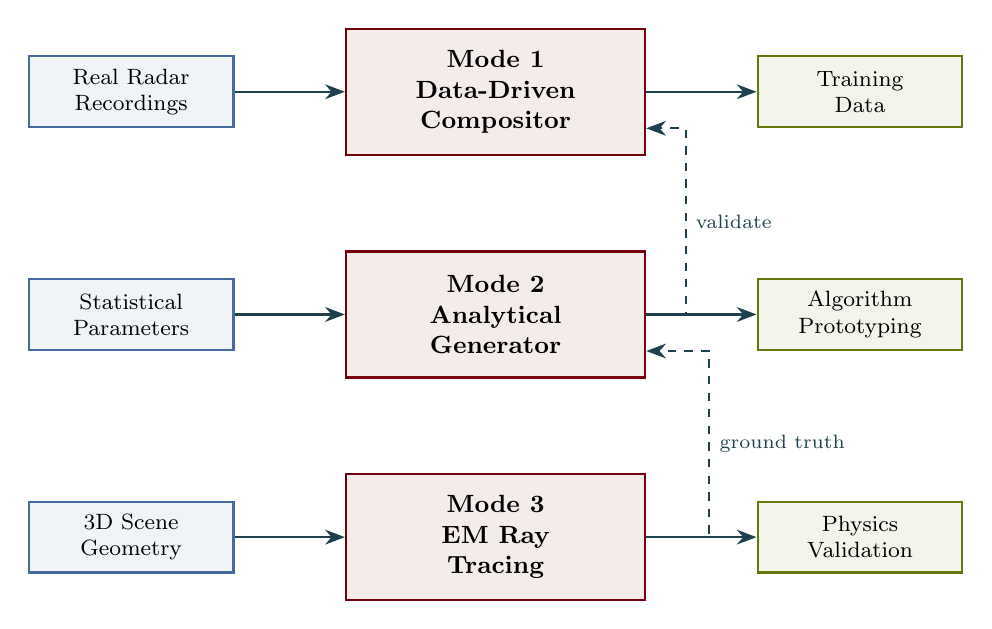
\begin{tikzpicture}[
    node distance=0.8cm and 1.2cm,
    mode/.style={rectangle, draw=Garnet, fill=Garnet!8, thick, minimum width=3.8cm, minimum height=1.6cm, align=center, font=\small\bfseries},
    data/.style={rectangle, draw=CBlue, fill=CBlue!8, thick, minimum width=2.6cm, minimum height=0.9cm, align=center, font=\footnotesize},
    output/.style={rectangle, draw=COlive, fill=COlive!8, thick, minimum width=2.6cm, minimum height=0.9cm, align=center, font=\footnotesize},
    arrow/.style={-{Stealth[length=2.5mm]}, thick, CDark},
    dasharrow/.style={-{Stealth[length=2.5mm]}, thick, CDark, dashed},
]

% Modes
\node[mode] (m1) {Mode 1\\Data-Driven\\Compositor};
\node[mode, below=1.2cm of m1] (m2) {Mode 2\\Analytical\\Generator};
\node[mode, below=1.2cm of m2] (m3) {Mode 3\\EM Ray\\Tracing};

% Inputs
\node[data, left=1.4cm of m1] (real) {Real Radar\\Recordings};
\node[data, left=1.4cm of m2] (params) {Statistical\\Parameters};
\node[data, left=1.4cm of m3] (scene) {3D Scene\\Geometry};

% Outputs
\node[output, right=1.4cm of m1] (train) {Training\\Data};
\node[output, right=1.4cm of m2] (proto) {Algorithm\\Prototyping};
\node[output, right=1.4cm of m3] (valid) {Physics\\Validation};

% Arrows
\draw[arrow] (real) -- (m1);
\draw[arrow] (params) -- (m2);
\draw[arrow] (scene) -- (m3);
\draw[arrow] (m1) -- (train);
\draw[arrow] (m2) -- (proto);
\draw[arrow] (m3) -- (valid);

% Cross-mode arrows
\draw[dasharrow] (m2.east) -- ++(0.5,0) |- node[right, pos=0.25, font=\scriptsize, text=CDark]{validate} (m1.east |- train.south);
\draw[dasharrow] (m3.east) -- ++(0.8,0) |- node[right, pos=0.25, font=\scriptsize, text=CDark]{ground truth} (m2.east |- proto.south);

\end{tikzpicture}
\end{document}
